\chapter{Benchmarking}
\label{ch:chapter1}


\section{Datasets}

\begin{figure}[h]
    \centering
    % First subfigure
    \begin{subfigure}[t]{0.49\textwidth}
        \centering
        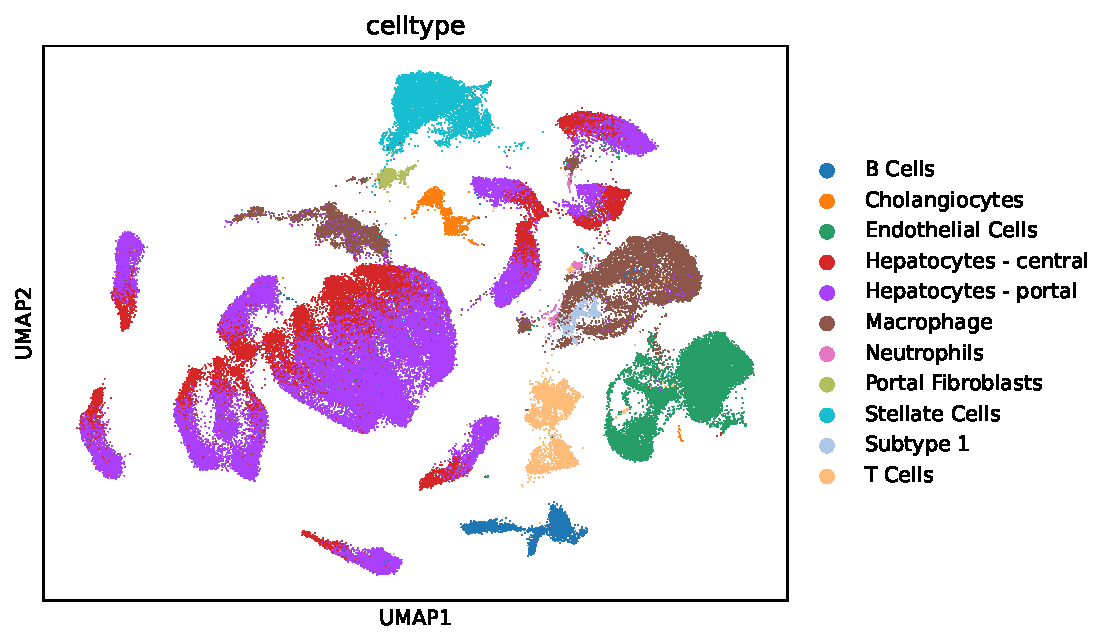
\includegraphics[width=\textwidth]{figures/nault_cell_umap.pdf}
        \caption{}
        \label{fig:figure1}
    \end{subfigure}%
    \hfill % Space between subfigures
    % Second subfigure
    \begin{subfigure}[t]{0.49\textwidth}
        \centering
        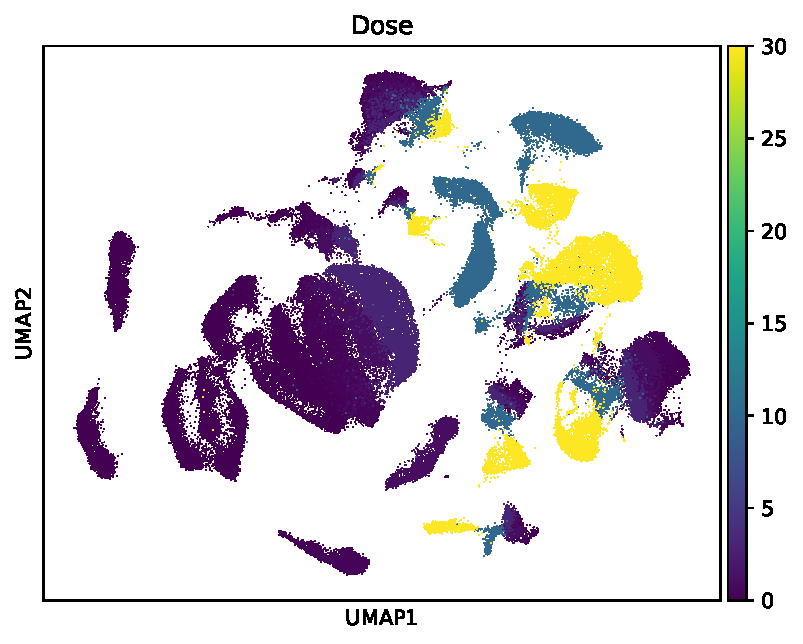
\includegraphics[width=.75\textwidth]{figures/nault_dose_umap.pdf}
        \caption{}
        \label{fig:figure2}
    \end{subfigure}%
    \hfill % Space between subfigures
    % Third subfigure
    \begin{subfigure}[b]{\textwidth}
        \centering
        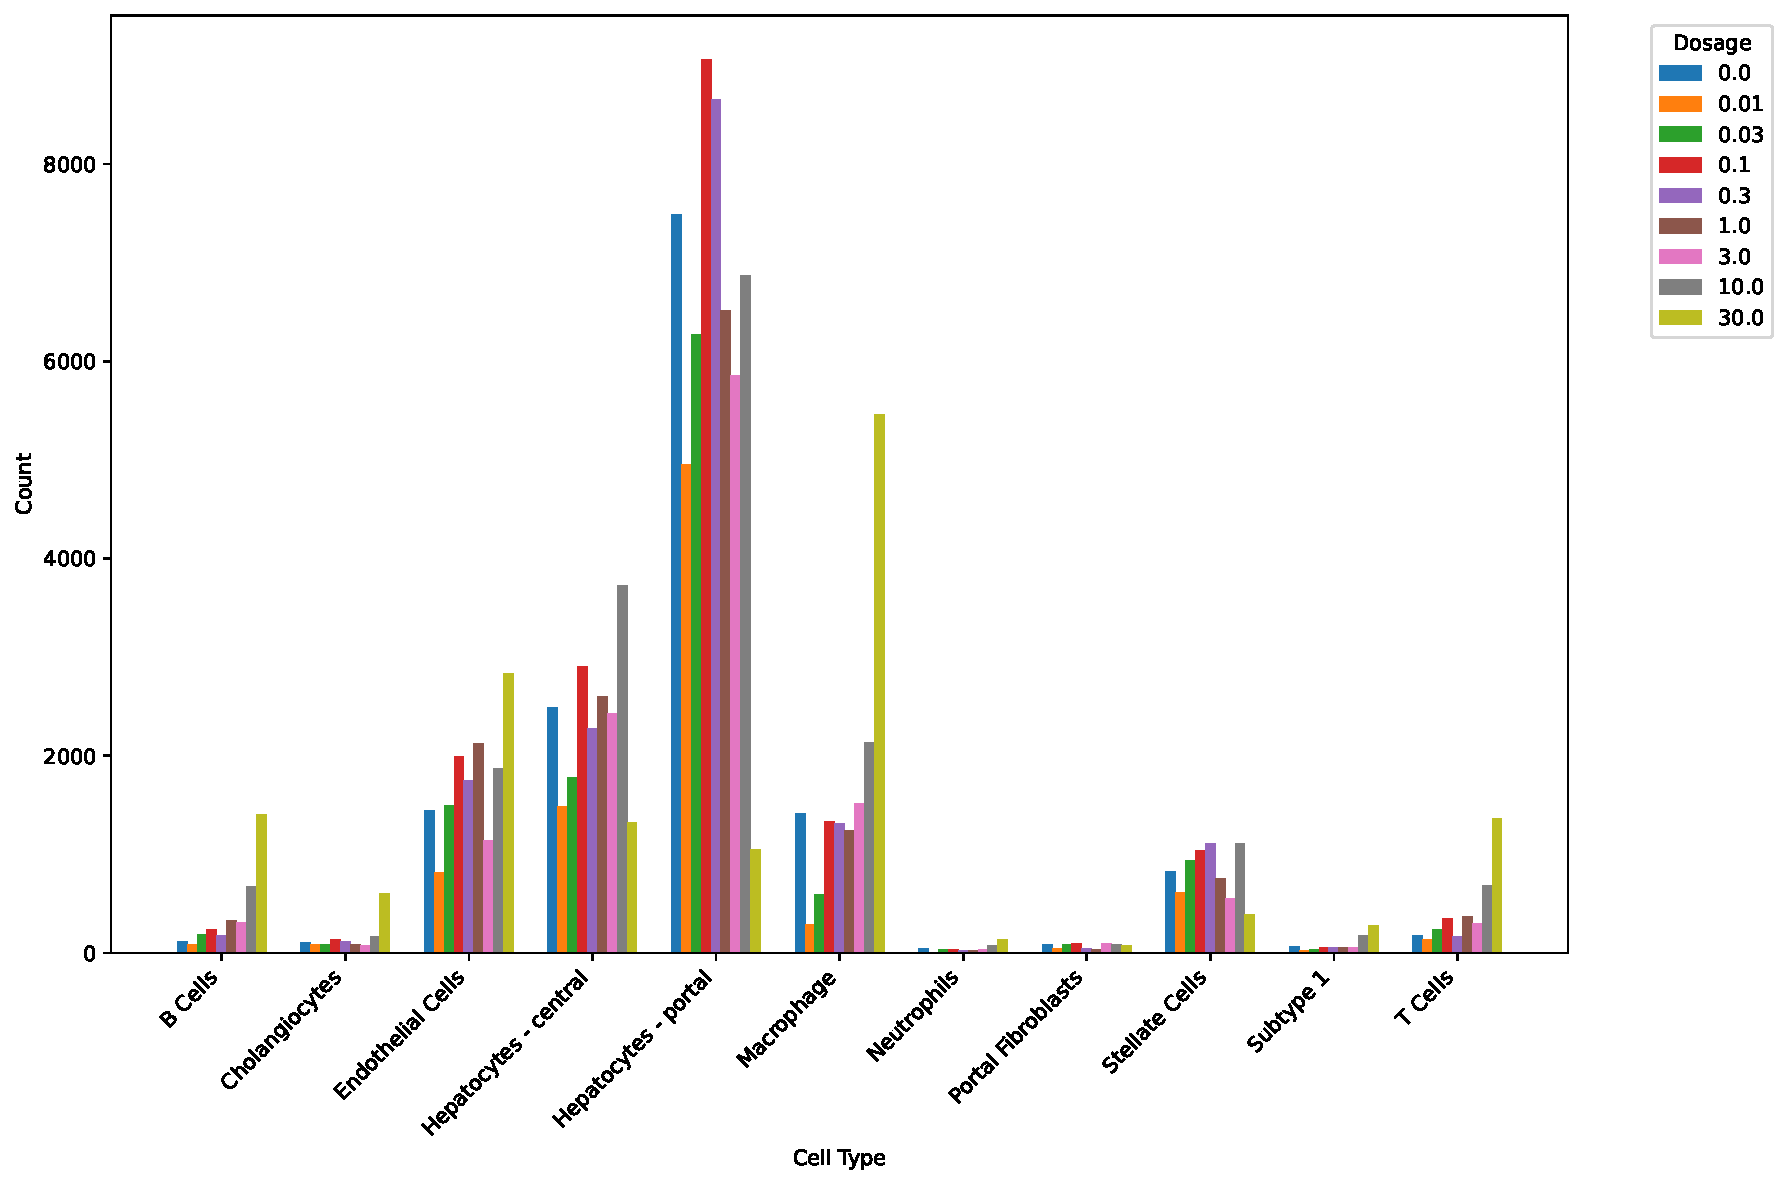
\includegraphics[width=.8\textwidth]{figures/nault_counts.pdf}
        \caption{}
        \label{fig:figure3}
    \end{subfigure}
    \caption{}
    \label{fig:combined}
\end{figure}


\begin{figure}[h]
    \centering
    % First subfigure
    \begin{subfigure}[t]{0.49\textwidth}
        \centering
        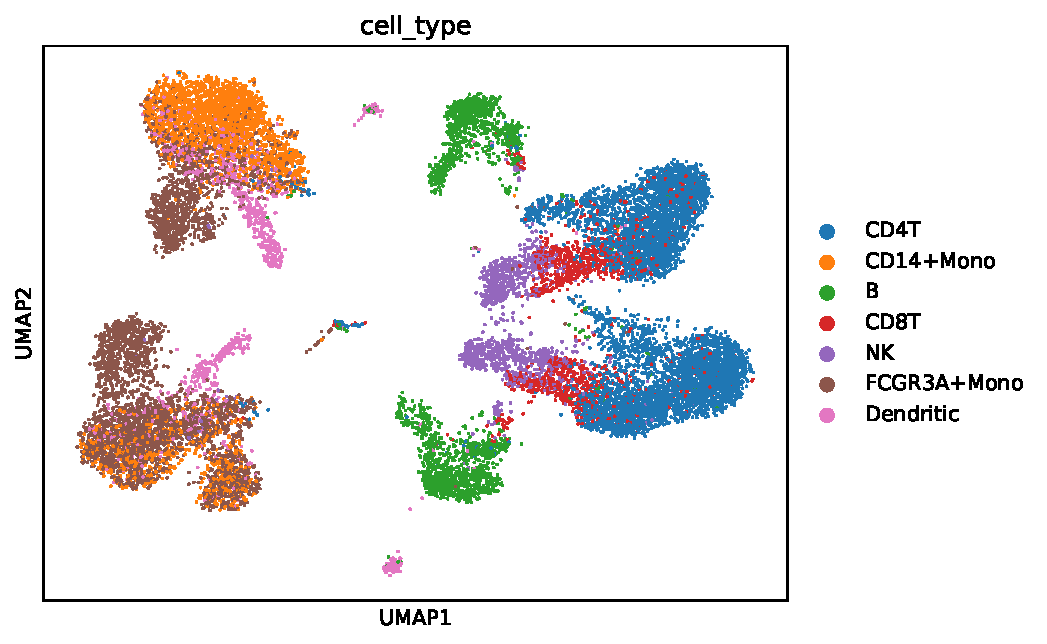
\includegraphics[width=\textwidth]{figures/pbmc_cell_umap.pdf}
        \caption{}
        \label{fig:figure1}
    \end{subfigure}%
    \hfill % Space between subfigures
    % Second subfigure
    \begin{subfigure}[t]{0.49\textwidth}
        \centering
        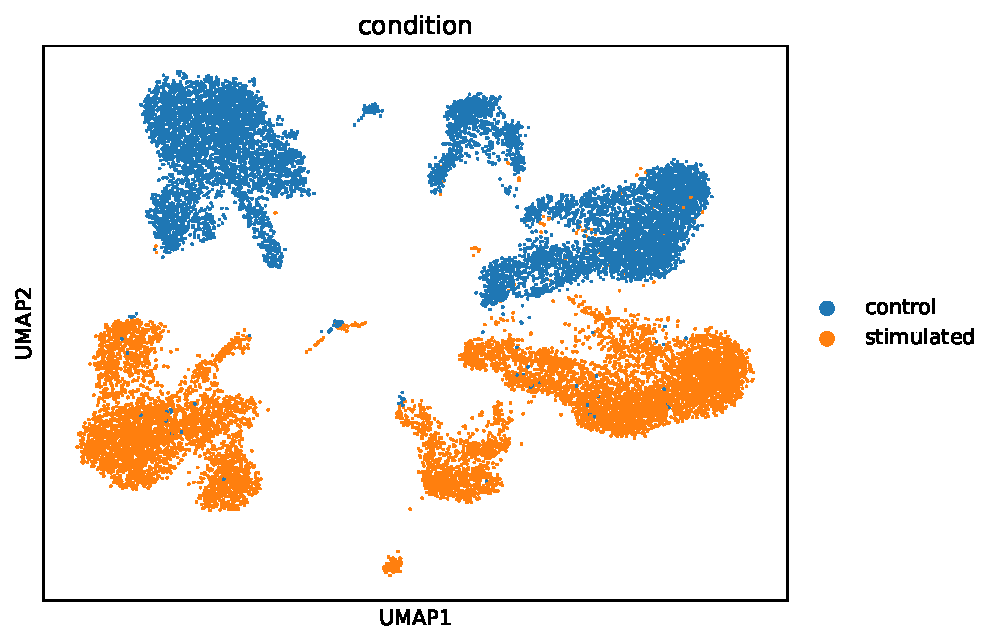
\includegraphics[width=.95\textwidth]{figures/pbmc_condtion_umap.pdf}
        \caption{}
        \label{fig:figure2}
    \end{subfigure}%
    \hfill % Space between subfigures
    % Third subfigure
    \begin{subfigure}[b]{\textwidth}
        \centering
        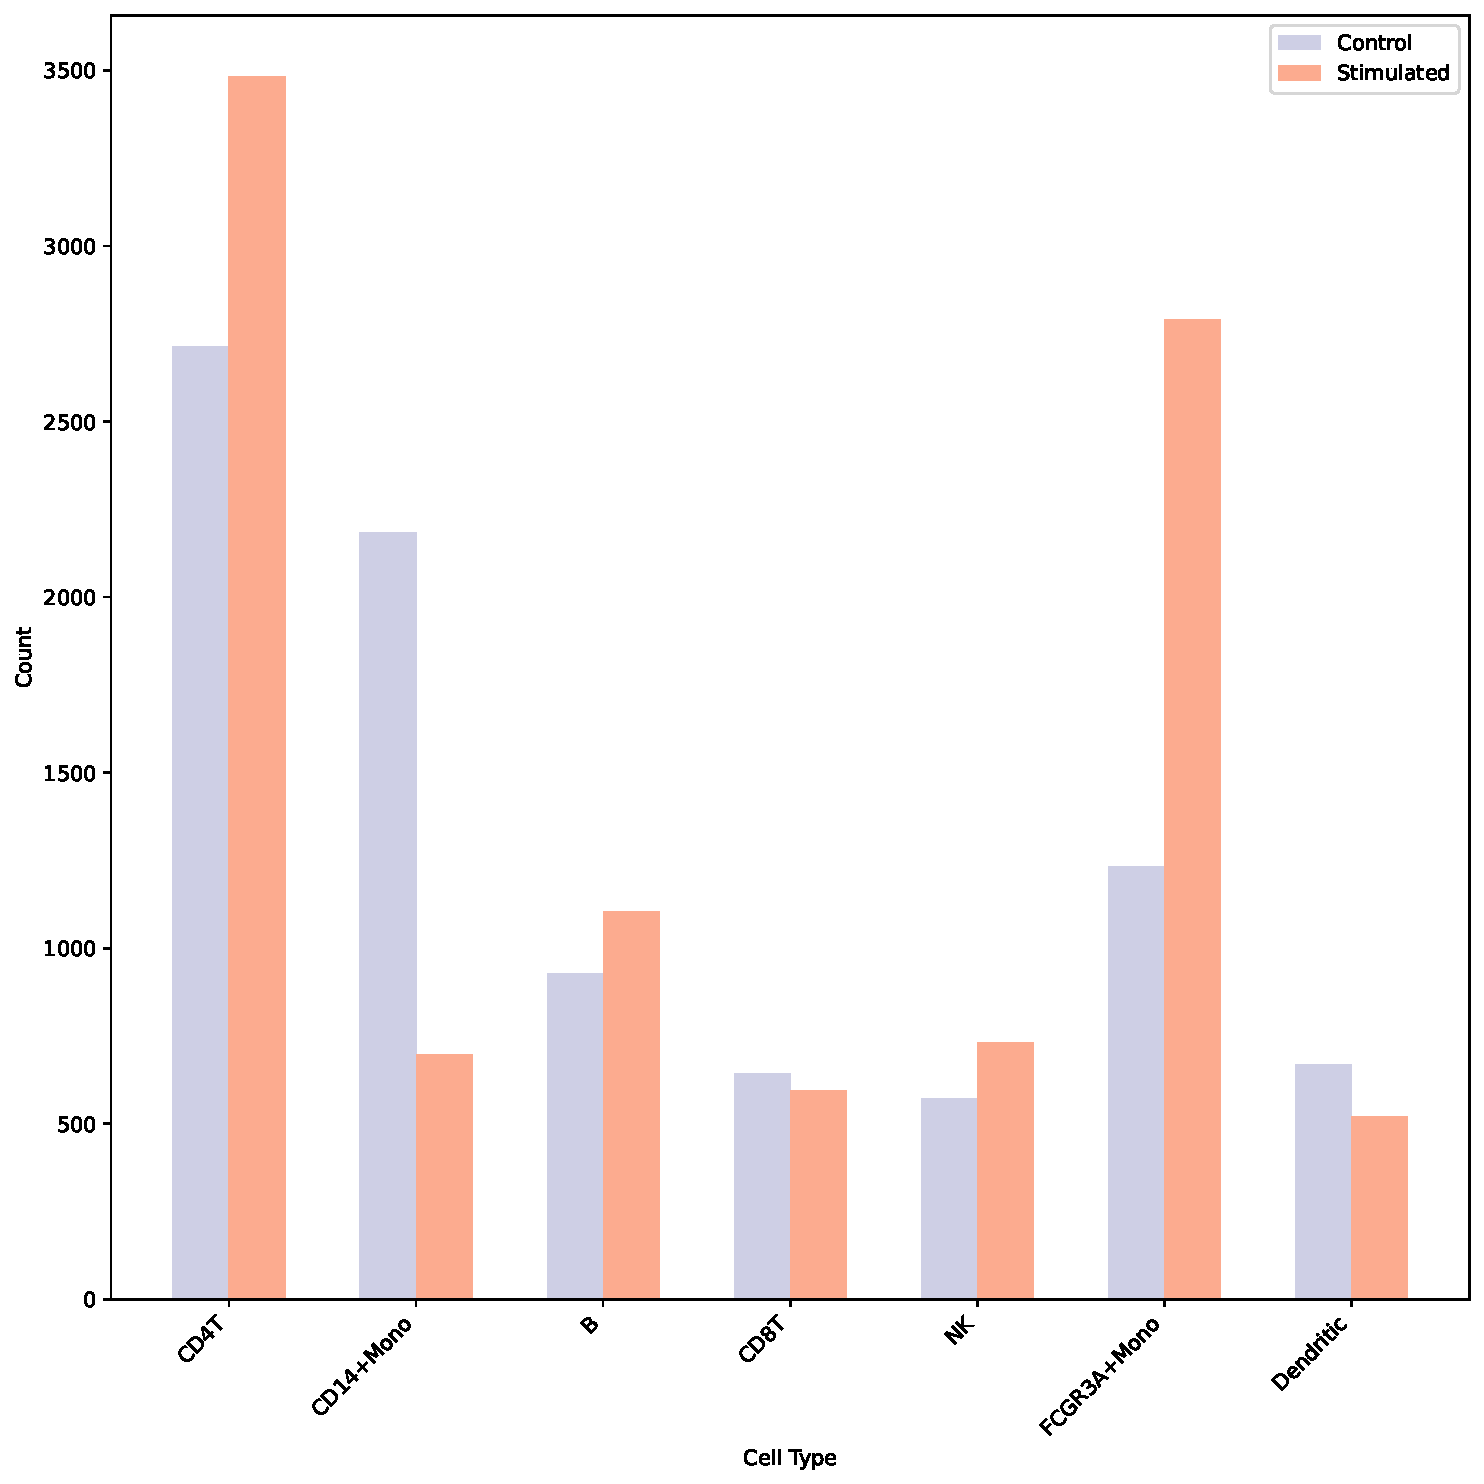
\includegraphics[width=.7\textwidth]{figures/pbmc_counts.pdf}
        \caption{}
        \label{fig:figure3}
    \end{subfigure}
    \caption{}
    \label{fig:combined}
\end{figure}